\documentclass{beamer}

\usepackage{amsmath}

\usetheme{AnnArbor}
\usecolortheme{crane}
\usefonttheme[onlymath]{serif}

\title{Deep Learning - Foundations and Concepts}
\subtitle{Chapter 18. Normalizing Flows}
\author{nonlineark@github}
\date{\today}

\begin{document}

\begin{frame}
    \titlepage
\end{frame}

\begin{frame}
    \frametitle{Outline}
    \tableofcontents
\end{frame}

\begin{frame}
    \frametitle{Normalizing flows}
    \begin{itemize}
        \item We define a distribution $p_{z}(z)$ over a latent variable $z$.
        \item And we use a deep neural network architecture to define an invertible function $x=f(z;w)$ that transforms the latent space into the data space.
        \item We can ensure that the overall function is invertible if we make each layer of the network invertible:
        \begin{itemize}
            \item $x=f^{A}(f^{B}(f^{C}(z)))$.
            \item $z=g^{C}(g^{B}(g^{A}(x)))$.
        \end{itemize}
    \end{itemize}
\end{frame}

\begin{frame}
    \frametitle{Normalizing flows}
    This approach to modelling a flexible distribution is called a normalizing flow because:
    \begin{itemize}
        \item The transformation of a probability distribution through a sequence of mappings is somewhat analogous to the flow of a fluid.
        \item The effect of the inverse mapping is to transform the complex data distribution into a normalized form, typically a Gaussian distribution.
    \end{itemize}
\end{frame}

\section{Coupling Flows}

\begin{frame}
    \frametitle{Real NVP}
    \begin{figure}
        \caption{A single layer of the real NVP normalizing flow model}
        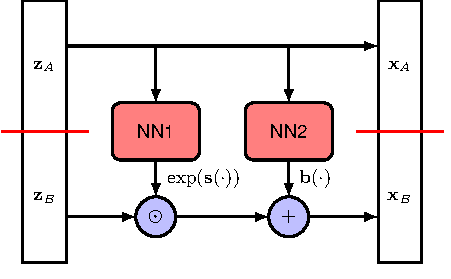
\includegraphics{Figure_1.pdf}
    \end{figure}
\end{frame}

\begin{frame}
    \frametitle{Real NVP}
    Real-valued non-volume-preserving (real NVP) partitions the latent variable $z\in\mathbb{R}^{D}$ and the output vector $x\in\mathbb{R}^{D}$ into two parts: $z=(z_{A},z_{B})$ and $x=(x_{A},x_{B})$, where $z_{A},x_{A}\in\mathbb{R}^{d}$. The transformation function is given by:
    \begin{align*}
        x_{A}&=z_{A} \\
        x_{B}&=\exp(s(z_{A};w))\odot{}z_{B}+b(z_{A};w)
    \end{align*}
    where $s(z_{A};w)$ and $b(z_{A};w)$ are the real-valued outputs of neural networks, and $\odot$ denotes element-wise multiplication of the two vectors.
\end{frame}

\begin{frame}
    \frametitle{Real NVP}
    The overall transformation is easily invertible:
    \begin{align*}
        z_{A}&=x_{A} \\
        z_{B}&=\exp(-s(x_{A};w))\odot(x_{B}-b(x_{A};w))
    \end{align*}
    The Jacobian matrix of this inverse mapping is given by:
    \begin{equation*}
        J=\begin{pmatrix}
            I_{d}&0 \\
            \frac{\partial{}z_{B}}{\partial{}x_{A}}&\mathrm{diag}(\exp(-s(x_{A};w)))
        \end{pmatrix}
    \end{equation*}
    We see that the Jacobian matrix is a lower triangular matrix, and its determinant is simply given by the product of the elements of $\exp(-s(x_{A};w))$.
\end{frame}

\begin{frame}
    \frametitle{Real NVP}
    \begin{figure}
        \caption{A double-layer structure where the roles of $z_{A}$ and $z_{B}$ are reversed in the second layer}
        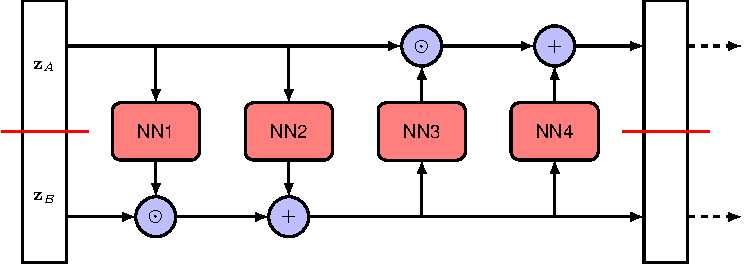
\includegraphics[width=0.8\textwidth]{Figure_2.pdf}
    \end{figure}
\end{frame}

\begin{frame}
    \frametitle{Coupling flows}
    The real NVP model belongs to a broad class of normalizing flows called coupling flows:
    \begin{align*}
        x_{A}&=z_{A} \\
        x_{B}&=h(z_{B},g(z_{A};w))
    \end{align*}
    where:
    \begin{itemize}
        \item $h(z_{B},g)$ is a function of $z_{B}$ that is efficiently invertible for any given value of $g$ and is called the coupling function.
        \item The function $g(z_{A};w)$ is called a conditioner and is typically represented by a neural network.
    \end{itemize}
\end{frame}

\section{Autoregressive Flows}

\begin{frame}
    \frametitle{Masked autoregressive flows}
    In masked autoregressive flows (MAFs), the transformation function from the latent space into the data space is given by:
    \begin{equation*}
        x_{d}=h(z_{d},g_{d}(x_{1:d-1};w_{d}))
    \end{equation*}
    where:
    \begin{itemize}
        \item $h$ is the coupling function, which is chosen to be easily invertible with respect to $z_{d}$.
        \item $g_{d}$ is the conditioner, which is typically represented by a deep neural network.
        \item $x_{1:d-1}$ denotes $x_{1},\hdots,x_{d-1}$.
    \end{itemize}
\end{frame}

\begin{frame}
    \frametitle{Masked autoregressive flows}
    The overall transformation is easily invertible:
    \begin{equation*}
        z_{d}=h^{-1}(x_{d},g_{d}(x_{1:d-1};w_{d}))
    \end{equation*}
    \begin{itemize}
        \item The inverse can be performed efficiently on modern hardware since $z_{1},\hdots,z_{D}$ can be evaluated in parallel.
        \item The Jocobian matrix is a lower-triangular matrix whose determinant can also be evaluated efficiently.
        \item However, sampling from this model must be done sequentially because the values of $x_{1},\hdots,x_{d-1}$ must be evaluated before $x_{d}$ can be computed.
    \end{itemize}
\end{frame}

\begin{frame}
    \frametitle{Inverse autoregressive flows}
    To avoid this inefficient sampling, we can instead define an inverse autoregressive flow (IAF) given by:
    \begin{equation*}
        x_{d}=h(z_{d},\tilde{g}_{d}(z_{1:d-1};w_d))
    \end{equation*}
    The inverse is given by:
    \begin{equation*}
        z_{d}=h^{-1}(x_{d},\tilde{g}_{d}(z_{1:d-1};w_d))
    \end{equation*}
    We see that:
    \begin{itemize}
        \item Sampling is now efficient since the evaluation of the elements $x_{1},\hdots,x_{D}$ can be performed in parallel.
        \item The Jocobian matrix is again a lower-triangular matrix whose determinant can be evaluated efficiently.
        \item The inverse calculations are intrinsically sequential and slow.
    \end{itemize}
\end{frame}

\section{Continuous Flows}

\begin{frame}
    \frametitle{Neural differential equations}
    Consider a residual network:
    \begin{equation*}
        z^{(t+1)}=z^{(t)}+f(z^{(t)};w)
    \end{equation*}
    where $t$ labels the layers in the network. Now we consider a small increment $\epsilon$ in the layer variable $t$:
    \begin{equation*}
        z^{(t+\epsilon)}=z^{(t)}+\epsilon{}f(z^{(t)};w)
    \end{equation*}
    Taking the limit $\epsilon\to{}0$, the hidden-unit activation vector becomes a function $z(t)$ of a continous variable $t$, and we can express the evolution of this vector through the network as a differential equation:
    \begin{equation*}
        \frac{\mathrm{d}z(t)}{\mathrm{d}t}=f(z(t);w)
    \end{equation*}
    where $t$ is often referred to as time.
\end{frame}

\begin{frame}
    \frametitle{Neural differential equations}
    If we denote the input to the network by the vector $z(0)$, then the output $z(T)$ is obtained by integration of the differential equation:
    \begin{equation*}
        z(T)=z(0)+\int_{0}^{T}f(z(t);w)\mathrm{d}t
    \end{equation*}
    This integral can be evaluated using standard numerical integration packages.
\end{frame}

\begin{frame}
    \frametitle{Neural differential equations}
    \begin{figure}
        \caption{Comparison of a conventional layered network with a neural differential equation}
        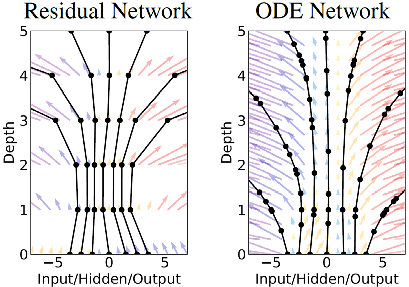
\includegraphics{Figure_5.pdf}
    \end{figure}
\end{frame}

\begin{frame}
    \frametitle{Neural ODE backpropagation}
    Let us assume that we are given a data set comprising values of the input vector $z(0)$ along with an associated output target vector and a loss function $L$ that depends on the output vector $z(T)$.
    \bigbreak
    One approach to training a neural ODE would be to use automatic differentiation to differentiate through all of the operations performed by the ODE solver during the forward pass. Although this is straightforward to do, it is costly from a memory perspective and is not optimal in terms of controlling numerical error.
\end{frame}

\begin{frame}
    \frametitle{Neural ODE backpropagation}
    For any two time values $0\le{}t_{1}\le{}t_{2}\le{}T$ and a network parameter vector $w$, we define a map $g^{t_{1}:t_{2}}_{w}:\mathbb{R}^{D}\to\mathbb{R}^{D}$, also known as the phase flow map of our neural ODE:
    \begin{itemize}
        \item There is a solution for our neural ODE whose graph passes through the point $(t_{1},z_{1})$ when the network parameter vector is $w$. Let's denote this solution by $\phi(t)$.
        \item Then $g^{t_{1}:t_{2}}_{w}(z_{1})$ is given by the value of this particular solution at $t_{2}$: $g^{t_{1}:t_{2}}_{w}(z_{1})=\phi(t_{2})$.
    \end{itemize}
\end{frame}

\begin{frame}
    \frametitle{Neural ODE backpropagation}
    Now our training objective is defined as:
    \begin{equation*}
        L(z_{T})=L(g^{0:T}_{w}(z_{0}))
    \end{equation*}
    It can be shown that:
    \begin{align*}
        \frac{\partial{}g^{0:T}_{w}(z(0))}{\partial{}w}&=\int_{0}^{T}\frac{\partial{}g^{t:T}_{w}(z(t))}{\partial{}z}\frac{\partial{}f(z(t);w)}{\partial{}w}\mathrm{d}t \\
        \frac{\partial{}L(w)}{\partial{}w}&=\int_{0}^{T}(\frac{\partial{}L(z(T))}{\partial{}z_{T}}\frac{\partial{}g^{t:T}_{w}(z(t))}{\partial{}z})\frac{\partial{}f(z(t);w)}{\partial{}w}\mathrm{d}t \\
        &=\int_{0}^{T}\frac{\partial{}(L\circ{}g^{t:T}_{w})(z(t))}{\partial{}z}\frac{\partial{}f(z(t);w)}{\partial{}w}\mathrm{d}t
    \end{align*}
\end{frame}

\begin{frame}
    \frametitle{Neural ODE backpropagation}
    Let $a(t)=\frac{\partial{}(L\circ{}g^{t:T}_{w})(z(t))}{\partial{}z}$, it can be shown that:
    \begin{equation*}
        \frac{\mathrm{d}a(t)}{\mathrm{d}t}=-a(t)\frac{\partial{f(z(t);w)}}{\partial{}z}
    \end{equation*}
    This is called the adjoint equation. The initial condition is given by:
    \begin{equation*}
        a(T)=\frac{\partial{}L(z(T))}{\partial{}z_{T}}
    \end{equation*}
    \href{https://ilya.schurov.com/post/adjoint-method/}{Further references}.
\end{frame}

\begin{frame}
    \frametitle{Neural ODE flows}
    If we define a base distribution over the input vector $p(z(0))$ then the neural ODE propagates this forward through time to give a distribution $p(z(t))$ for each value of $t$, leading to a distribution over the output vector $p(z(T))$. It can be shown that the transformation for the density can be evaluated by integrating a differential equation given by:
    \begin{equation*}
        \frac{\mathrm{d}\log{}p(z(t))}{\mathrm{d}t}=-\mathrm{tr}(\frac{\partial{}f(z(t);w)}{\partial{}z})
    \end{equation*}
    \href{https://arxiv.org/pdf/1806.07366}{Further references}.
\end{frame}

\begin{frame}
    \frametitle{Neural ODE flows}
    \begin{figure}
        \caption{Illustration of a continuous normalizing flow}
        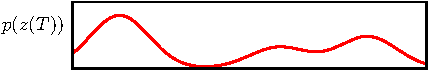
\includegraphics{Figure_6_a.pdf}
        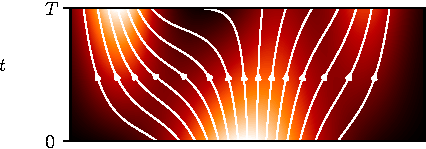
\includegraphics{Figure_6_b.pdf}
        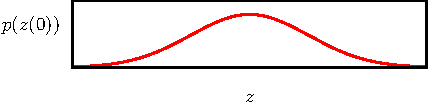
\includegraphics{Figure_6_c.pdf}
    \end{figure}
\end{frame}

\end{document}